\documentclass[11pt]{article}
	
%%%%%%%%%%%%%%%%%%%%%%%%%%%%%%%%%%%%%%%%%%%%%%%%%%%%%%%%%%%%%%%%%%%%%%
%\pdfminorversion=4
% NOTE: To produce blinded version, replace "0" with "1" below.
\newcommand{\blind}{0}

%%%%%%% IISE Transactions margin specifications %%%%%%%%%%%%%%%%%%%
% DON'T change margins - should be 1 inch all around.
\addtolength{\oddsidemargin}{-.5in}%
\addtolength{\evensidemargin}{-.5in}%
\addtolength{\textwidth}{1in}%
\addtolength{\textheight}{1.3in}%
\addtolength{\topmargin}{-.8in}%
\makeatletter
\renewcommand\section{\@startsection {section}{1}{\z@}%
                                   {-3.5ex \@plus -1ex \@minus -.2ex}%
                                   {2.3ex \@plus.2ex}%
                                   {\normalfont\fontfamily{phv}\fontsize{16}{19}\bfseries}}
\renewcommand\subsection{\@startsection{subsection}{2}{\z@}%
                                     {-3.25ex\@plus -1ex \@minus -.2ex}%
                                     {1.5ex \@plus .2ex}%
                                     {\normalfont\fontfamily{phv}\fontsize{14}{17}\bfseries}}
\renewcommand\subsubsection{\@startsection{subsubsection}{3}{\z@}%
                                    {-3.25ex\@plus -1ex \@minus -.2ex}%
                                     {1.5ex \@plus .2ex}%
                                     {\normalfont\normalsize\fontfamily{phv}\fontsize{14}{17}\selectfont}}
\makeatother
%%%%%%%%%%%%%%%%%%%%%%%%%%%%%%%%%%%%%%%%%%%%%%%%%%%%%%%%%%%%%%%%%%%%%%%%%

%%%%% IISE Transactions package list %%%%%%%%%%%%%%%%%%%%%%%%%%%%%%%%%%%%%%
\usepackage{amsmath}
\usepackage{amsfonts}
\usepackage{mathtools}
\usepackage{graphicx}
\usepackage{enumerate}
\usepackage{natbib} %comment out if you do not have the package
\usepackage{url} % not crucial - just used below for the URL
%%%%%%%%%%%%%%%%%%%%%%%%%%%%%%%%%%%%%%%%%%%%%%%%%%%%%%%%%%%%%%%%%%%%%%%

%%%%% Author package list and commands %%%%%%%%%%%%%%%%%%%%%%%%%%%%%%%%%%%%%%%%%%%%%
%%%%% Here are some examples %%%%%%%%%%%%%%
%	\usepackage{amsfonts, amsthm, latexsym, amssymb}
%	\usepackage{lineno}
%	\newcommand{\mb}{\mathbf}
%%%%%%%%%%%%%%%%%%%%%%%%%%%%%%%%%%%%%%%%%%%%%%%%%%%%%%%%%%%%%%%%%%%%%%%%%%%%%%

\begin{document}
	
		%%%%%%%%%%%%%%%%%%%%%%%%%%%%%%%%%%%%%%%%%%%%%%%%%%%%%%%%%%%%%%%%%%%%%%%%%%%%%%
	\def\spacingset#1{\renewcommand{\baselinestretch}%
		{#1}\small\normalsize} \spacingset{1}
	%%%%%%%%%%%%%%%%%%%%%%%%%%%%%%%%%%%%%%%%%%%%%%%%%%%%%%%%%%%%%%%%%%%%%%%%%%%%%%
	
	\if0\blind
	{
		\title{\bf Simulation-guided Data Assimilation for Kinetics Modeling of Potassium Channel Isoforms in Mouse Cardiomyocytes}
		\author{Haedong Kim $^a$, Hui Yang $^a$, Andrew R. Ednie $^b$, and Eric S. Bennett $^b$ \\
		$^a$ Department of Industrial and Manufacturing Engineering, \\
		The Pennsylvania State University, State College, PA USA \\
        $^b$ Department of Neuroscience, Cell Biology, and Physiology, \\
        Wright State University, City, OH USA}
		\date{}
		\maketitle
	} \fi
	
	\if1\blind
	{
        \title{\bf \emph{IISE Transactions} \LaTeX \ Template}
		\author{Author information is purposely removed for double-blind review}
		
\bigskip
		\bigskip
		\bigskip
		\begin{center}
			{\LARGE\bf \emph{IISE Transactions} \LaTeX \ Template}
		\end{center}
		\medskip
	} \fi
	\bigskip
		
\begin{abstract}
Aberrant activities of voltage-gated potassium (K\textsubscript{v}) channels can cause fatal heart disease such as long QT syndrome. In our recent investigation on a disease-related perturbation, reduced glycosylation in cardiomyocytes, significant reduction in K\textsuperscript{+} currents was observed. Among major cardiac voltage-gated ion channels (VGIC), K\textsubscript{v} channels have a distinctive feature: various isoforms generate their own unique currents contributing to different phases of repolarization of cardiac action potential (AP). On the other hand, the dominant isoform is responsible for Na\textsuperscript{+} and Ca\textsuperscript{2+} currents. Because only the sum of these K\textsuperscript{+} currents (I\textsubscript{Ksum}) can be recorded in experiments, data analytical methods are necessary to estimate the properties of individual K\textsuperscript{+} currents and their effects on the behaviors of the cardiomyocyte. However, traditional approaches estimate only one property, the shape of individual K\textsuperscript{+} currents, from a single I\textsubscript{Ksum} recording rather than analyzing I\textsubscript{Ksum} recordings from the same cell with different conditions. These approaches assume the functional form of the shape of K\textsuperscript{+} currents and search the shape parameters in the current functions that the sum of estimated currents has the best fit with a single I\textsubscript{Ksum} recording. It does not provide information about underlying kinetics of the currents at the cellular level. First, computer models of K\textsuperscript{+} currents are designed with parameters that control the kinetic rates and, in turn, determine the currents. Second, we develop fractional factorial designs to identify the parameters that have significant impacts on the current shapes. Third, we design model calibration as nonlinear optimization that couple the \textit{in-silico} model and \textit{in-vitro} I\textsubscript{Ksum} recordings by minimizing discrepancies between them. Further, we develop a graphical user interface (GUI) application to make the proposed framework accessible for researchers and patricians without engineering backgrounds. We apply the proposed framework to our data, and the experimental results show that the data assimilation method can estimate differences in kinetic rate between the control and experiment groups. This method has strong potential to pave a new way to analyze K\textsuperscript{+} currents.
\end{abstract}
		
\noindent%
{\it Keywords:} Potassium channels, kinetics modeling, data assimilation, model calibration, reduced glycosylation

%\newpage
\spacingset{1.5} % DON'T change the spacing!


\section{Introduction} \label{s:intro}
\begin{itemize}
    \item \textbf{Motivation:} Aberrant activities of voltage-gated potassium (K\textsubscript{v}) channels can cause fatal heart disease such as long QT syndrome. In our recent investigation on a disease-related perturbation, reduced glycosylation in cardiomyocytes, significant reduction in K\textsuperscript{+} currents was observed. Among major cardiac voltage-gated ion channels (VGIC), K\textsubscript{v} channels have a distinctive feature: various isoforms generate their own unique currents contributing to different phases of repolarization of cardiac action potential (AP). On the other hand, the dominant isoform is responsible for Na\textsuperscript{+} and Ca\textsuperscript{2+} currents. Because only the sum of these K\textsuperscript{+} currents (I\textsubscript{Ksum}) can be recorded in experiments, data analytical methods are necessary to estimate the properties of individual K\textsuperscript{+} currents and their effects on the behaviors of the cardiomyocyte.
    \item \textbf{Gaps \& Needs:} However, traditional approaches estimate only one property, the shape of individual K\textsuperscript{+} currents, from a single I\textsubscript{Ksum} recording rather than analyzing I\textsubscript{Ksum} recordings from the same cell with different conditions. These approaches assume the functional form of the shape of K\textsuperscript{+} currents and search the shape parameters in the current functions that the sum of estimated currents has the best fit with a single I\textsubscript{Ksum} recording. It does not provide information about underlying kinetics of the currents at the cellular level.
    \item \textbf{Objective:} In this paper, we present a novel framework of data assimilation method that delineates kinetics of K\textsubscript{v} isoforms from I\textsubscript{Ksum} recordings based on computer models of K\textsuperscript{+} currents that simulate underlying biophysics of the currents. As opposed to the traditional data-driven curve fitting method, the proposed biophysics-driven method estimates the cellular-level kinetics of K\textsubscript{v} isoforms.
    \item \textbf{Approach:} First, computer models of K\textsuperscript{+} currents are designed with parameters that control the kinetic rates and, in turn, determine the currents. Second, we develop fractional factorial designs to identify the parameters that have significant impacts on the current shapes. Third, we design model calibration as nonlinear optimization that couple the in-silico model and in-vivo I\textsubscript{Ksum} recordings by minimizing discrepancies between them. Further, we develop a graphical user interface (GUI) application to make the proposed framework accessible for researchers and patricians without engineering backgrounds.
    \item \textbf{Experiment \& Performance} We apply the proposed framework to our data, and the experimental results show that the data assimilation method can estimate differences in kinetic rate between the control and experiment groups.
    \item \textbf{Significance/Contributions} 1) We model the underlying kinetics of observed currents based on biophysical principles rather than curve-fitting methods. 2) The calibration process includes multiple protocols rather than a single protocol, resulting in comprehensive cellular-level modeling. 3) Our method provides differences in channel kinetics given the disease-related perturbation, such as reduced glycosylation. 
\end{itemize}

\begin{figure}
    \centering
    \includegraphics{figs/overall_diagram2.pdf}
    \caption{Caption}
    \label{fig:framework_diagram}
\end{figure}

\section{Methods} \label{s:methods}

\subsection{\emph{Computer Models of Potassium Channel Isoforms}} \label{s:methods.1}
Computer models mouse ventricular cardiomyocytes simulate important biophysical properties of ion channels and molecular dynamics in producing the AP. In this paper, the AP is modeled as a differential equation of transmembrane currents and stimulus current I\textsubscript{stim} as below in Equation~\ref{eq:ap} where $C_{m}$ is the membrane capacitance, $t$ is time.
\begin{equation}
    \label{eq:ap}
    \begin{split}
    -C_{m}\frac{dV}{dt} &= \mathrm{I}_{\mathrm{CaL}}+\mathrm{I}_{\mathrm{p}(Ca)}+\mathrm{I}_{\mathrm{NaCa}}+\mathrm{I}_{\mathrm{Cab}}+\mathrm{I}_{\mathrm{Na}}+\mathrm{I}_{\mathrm{Nab}}+\mathrm{I}_{\mathrm{NaK}}+\mathrm{I}_{\mathrm{Cl},Ca} \\
    &+\mathrm{I}_{\mathrm{Kto}}+\mathrm{I}_{\mathrm{Kslow1}}+\mathrm{I}_{\mathrm{Kslow2}}+\mathrm{I}_{\mathrm{Kss}}+\mathrm{I}_{\mathrm{Ks}}+\mathrm{I}_{\mathrm{Kr}}+\mathrm{I}_{\mathrm{K1}}+\mathrm{I}_{\mathrm{stim}}
    \end{split}
\end{equation}
There are 15 transmembrane currents in this AP model: the L-type calcium current (I\textsubscript{CaL}), the calcium pump current (I\textsubscript{p(Ca)}), the Na\textsuperscript{+}/Ca\textsuperscript{2+} exchange current (I\textsubscript{NaCa}), the calcium background current (I\textsubscript{Cab}), the fast Na\textsuperscript{+} current (I\textsubscript{Na}), the background Na\textsuperscript{+} current (I\textsubscript{Nab}), the Na\textsuperscript{+}/K\textsuperscript{+} pump current (I\textsubscript{NaK}), the Ca\textsuperscript{2+}-activated Cl\textsuperscript{-} current (I\textsubscript{Cl,Ca}), the rapidly inactivating transient outward K\textsuperscript{+} current (I\textsubscript{Kto}), the two ultra-rapidly activating delayed rectifier K\textsuperscript{+} currents (I\textsubscript{Kslow1} and I\textsubscript{Kslow2}), the non-inactivating steady-state K\textsuperscript{+} current (I\textsubscript{Kss}), the slow delayed rectifier K\textsuperscript{+} current (I\textsubscript{Ks}), the rapid delayed rectifier K\textsuperscript{+} current (I\textsubscript{Kr}), and the time independent K\textsuperscript{+} current (I\textsubscript{K1}).

The three types of K\textsuperscript{+} currents have larger magnitude compared to the other K\textsuperscript{+} currents: the rapidly inactivating transient outward K\textsuperscript{+} currents (I\textsubscript{Kto,f} and/or I\textsubscript{Kto,s}), the delayed rectifier K\textsuperscript{+} currents (I\textsubscript{Kslow1} and I\textsubscript{Kslow2}), and the non-inactivating steady-state K\textsuperscript{+} current (I\textsubscript{Kss}). The rapidly inactivating transient outward currents have two components I\textsubscript{Kto,f} and I\textsubscript{Kto,s}, but the later is essentially absent in apex cardiomyocytes. We only include I\textsubscript{Kto,f} in I\textsubscript{Kto}, because we focus on apex myocytes in this investigation. However, the transient outward current can be easily modified according to the region of ventricular cardiomyocytes. Therefore, we model K\textsubscript{v} isoforms that conduct these dominant currents: K\textsubscript{v}4.2 (I\textsubscript{Kto}), K\textsubscript{v}1.5 (I\textsubscript{Kslow1}), K\textsubscript{v}2.1 (I\textsubscript{Kslow2}), and K\textsubscript{2P} family (I\textsubscript{Kss}). \textbf{Figure~\ref{fig:kcurrent_example}B} illustrates the shape of the primary K\textsuperscript{+} currents and their contribution to the I\textsubscript{Ksum} given the protocol in \textbf{Figure~\ref{fig:kcurrent_example}A} that applies 0 mV voltage step from holding potential -70 mV from time $t^{(h)}$ to $t^{(e)}$. \textbf{Figure~\ref{fig:kcurrent_example}C} and \textbf{D} show a range of protocols and consequent change in I\textsubscript{Ksum}. Because of their shape, I\textsubscript{Kss} is assumed as a constant and the other currents an exponential function in the traditional data-driven curve-fitting approach. In this approach, K\textsuperscript{+} current can be defined by Equation~\ref{eq:expl_fitting} with the shape parameters such as amplitude $\mathrm{A}_{i}$ and time constant $\tau_{i}$ for $i \in \{\mathrm{Kto}, \mathrm{Kslow1}, \mathrm{Kslow2}, \mathrm{Kss}\}$, and a set of them is estimated that have the best fit with experimental I\textsubscript{Ksum} data.
\begin{figure}[!ht]
    \centering
    \includegraphics{figs/exemplary_kv_currents.pdf}
    \caption{Example of voltage-clamp K\textsuperscript{+} currents. (A) Voltage step of 0 mV from holding potential -70 mV. (B) Dominant K\textsuperscript{+} currents and their contributions to I\textsubscript{Ksum}. (C) Range of protocols from -50 to 50 mV from holding potential -70 mV and (D) consequent K\textsuperscript{+} current traces.}
    \label{fig:kcurrent_example}
\end{figure}
\begin{equation}
    \label{eq:expl_fitting}
    \mathrm{I}_{\mathrm{Ksum}} = \mathrm{A}_{\mathrm{Kto}}e^{-t/\tau_{\mathrm{Kto}}} + \mathrm{A}_{\mathrm{Kslow1}}e^{-t/\tau_{\mathrm{Kslow1}}} + \mathrm{A}_{\mathrm{Kslow2}}e^{-t/\tau_{\mathrm{Kslow2}}} +  \mathrm{A}_{\mathrm{Kss}}
\end{equation}

Unlike the simple current functions, computer models of K\textsubscript{v} isoforms can simulate detailed gating kinetics. We developed them with Hodgkin-Huxley modeling that has two gating variables controlling conductance. For example, K\textsubscript{v} isoforms that conducts current I\textsubscript{K} can be defined by Equation~\ref{eq:hh_ex}
\begin{equation}
    \label{eq:hh_ex}
    \mathrm{I}_{\mathrm{K}} = G_{\mathrm{K}}a^{n}i^{m}(V-E_{\mathrm{K}})
\end{equation}
where $G_{\mathrm{K}}$ is the maximum conductance, $a^{n}$ and $i^{m}$ are the gating variables for $n,m \in \mathbb{N}$, $V$ is the transmembrane potential, and $E_{\mathrm{K}}$ is the K\textsuperscript{+} Nernst potential. $V-E_{\mathrm{K}}$ is the driving force of the ion movement. Important components in this equation are the gating variables $a$ and $i$, representing the fraction of activation and recovery from inactivation of the channel where $a,i \in [0,1]$. These processes are governed by first-order kinetics and its voltage-dependent transition rates $\alpha$ and $\beta$. $\alpha$ is the rate at which a gate in closed state opens, whereas $\beta$ is the rates at which a gate in open state closes. Equation~\ref{eq:gv} shows a schematic relationship of this gating kinetics.
\begin{align}
    \label{eq:gv}
    (1-a)&\xrightleftharpoons[\beta_{a}]{\alpha_{a}}a & (1-i)&\xrightleftharpoons[\beta_{i}]{\alpha_{i}}i
\end{align}

The two biophysical processes can be modeled using differential equations in two ways as follows:
\begin{align}
    \frac{da}{dt} &=\alpha_{a}(1-a)-\beta_{a}a   &\frac{di}{dt} &=\alpha_{i}(1-i)-\beta_{i}i \\
    \frac{da}{dt} &= \frac{a_{\infty}-a}{\tau_{a}}  &\frac{di}{dt} &= \frac{i_{\infty}-i}{\tau_{i}}
\end{align}
where $a_{\infty}$ and $i_{\infty}$ are the steady-state values to which $a$ and $b$ converge; $\tau_{a}$ and $\tau_{i}$ are time constants determine the convergence speed defined by
\begin{align}
    a_{\infty} &= \frac{\alpha_{a}}{\alpha_{a}+\beta_{a}} & i_{\infty} &=  \frac{\alpha_{i}}{\alpha_{i}+\beta_{i}} \\
    \tau_{a} &= \frac{1}{\alpha_{a}+\beta_{a}} & \tau_{i} &= \frac{1}{\alpha_{i}+\beta_{i}}
\end{align}
The steady-state values and time constants can be defined directly by functions of voltage without transition rates in some cases. These voltage-dependent functions, such as transition rates, steady states, or time constants, have parameters that control the behavior of the kinetics of an ion channel.

\subsubsection{In-silico Modeling of K\textsubscript{v}4.2 (I\textsubscript{Kto})}
The rapidly inactivating transient outward current I\textsubscript{Kto}, conducted through K\textsubscript{v}4.2, is characterized by a sharp upstroke during activation and subsequent rapid inactivation. It mainly contributes to the peak at the very beginning of activation in I\textsubscript{Ksum}. I\textsubscript{Kto} is defined by
\begin{align}
    &\mathrm{I}_{\mathrm{Kto}} = G_{\mathrm{Kto}}a_{\mathrm{Kto}}^{3}i_{\mathrm{Kto}}(V-E_{\mathrm{K}}) \\
    &\frac{da_{\mathrm{Kto}}}{dt} = \alpha_{a}(1-a_{\mathrm{Kto}}) - \beta_{a}a_{\mathrm{Kto}} \\
    &\frac{di_{\mathrm{Kto}}}{dt} = \alpha_{i}(1-i_{\mathrm{Kto}}) - \beta_{i}i_{\mathrm{Kto}} \\
    &\alpha_{a} = p_{7}e^{p_{5}(V+p_{1})} \label{eq:ikto_alpha1} \\
    &\beta_{a}= p_{8}e^{-p_6(V+p_{1})} \\
    &\alpha_{i} = \frac{p_{9}e^{-(V+p_{2})/p_{4}}}{1+p_{10}e^{-(V+p_{2}+p_{3})/p_{4}}} \\
    & \beta_{i} = \frac{p_{11}e^{(V+p_{2}+p{3})/p_{4}}}{1+p_{12}e^{(V+p_{2}+p_{3})/p_{4}}} \label{eq:ikto_beta2}
\end{align}
There are two gating variables $a_{\mathrm{Kto}}$ and $i_{\mathrm{Kto}}$ responsible for activation and inactivation, respectively. Their kinetics are governed by transition-rate functions from Equation~\ref{eq:ikto_alpha1} to Equation~\ref{eq:ikto_beta2}. Parameters $p_{i}$ for $i=\{1, 2, \dots, 12\}$ in these equations act like ``knobs'', allowing to control the behavior of the I\textsubscript{Kto} model. \textbf{Figure~\ref{fig:kinetic_iktof}} shows a representative example of the relationship between the transition-rate functions and the channel kinetics, given the specific value of $p_{i}$. In general, the transition rates for inactivation gates change more rapidly and have smaller ranges than for activation, which results in a drastic slope in the steady-state curve and a large time constant.
\begin{figure}[!ht]
    \centering
    \includegraphics{figs/kinetic_iktof.pdf}
    \caption{Example of the behavior of the transition-rate functions with changes in voltage, given specific values of parameters that govern kinetics of I\textsubscript{Kto}.}
    \label{fig:kinetic_iktof}
\end{figure}

\subsubsection{In-silico Modeling of K\textsubscript{v}1.5 (I\textsubscript{Kslow1}), K\textsubscript{v}2.1 (I\textsubscript{Kslow2}) and K\textsubscript{2P} (I\textsubscript{Kss})}
There are two major delayed rectifier currents in mouse ventricular cardiomyocytes that are very rapidly activating: I\textsubscript{Kslow1} and I\textsubscript{Kslow2}, which are conducted through K\textsubscript{v}1.5 and K\textsubscript{v}2.1, respectively. As shown in \textbf{Figure~\ref{fig:kcurrent_example}}, both rectifier currents inactivate slower and have smaller magnitude than I\textsubscript{Kto}, but I\textsubscript{Kslow2} decays more gradually than I\textsubscript{Kslow1}. The non-inactivating steady-state current, which conducted through K\textsubscript{2P} family, remains constant during the voltage-clamp recording. These three currents collectively address the most part of the decaying phase of I\textsubscript{Ksum}. We assume that I\textsubscript{Kslow1} and I\textsubscript{Kslow2} have the same activation gating variable, and I\textsubscript{Kss} has similar activation behavior with a slightly different rate to keep the model as simple as possible to reduce the structural risk of overfitting.

I\textsubscript{Kslow1} is modeled without transition-rate functions as opposed to I\textsubscript{Kto}. Its gating variables, activation $a_{\mathrm{Kslow1}}$, and inactivation $i_{\mathrm{Kslow1}}$ are defined directly by steady-state ($a_{ss}$ and $i_{ss}$) and time-constant functions ($\tau_{a}^{(1)}$ and $\tau_{i}^{(1)}$) as follows.
\begin{align}
    &\mathrm{I}_{\mathrm{Kslow1}} = G_{\mathrm{Kslow1}}a_{\mathrm{Kslow1}}i_{\mathrm{Kslow1}}(V-E_{\mathrm{K}}) \\
    &\frac{da_{\mathrm{Kslow1}}}{dt} = \frac{a_{ss}-a_{\mathrm{Kslow1}}}{\tau_{a}^{(1)}} \\
    &\frac{di_{\mathrm{Kslow1}}}{dt} = \frac{i_{ss}-i_{\mathrm{Kslow1}}}{\tau_{i}^{(1)}} \\
    &a_{ss} = \frac{1}{1+e^{-(V+p_{1})/p_{4}}} \\
    &i_{ss} = \frac{1}{1+e^{(V+p_{2})/p_{5}}} \\
    &\tau_{a}^{(1)} = \frac{p_{7}}{e^{p_{6}(V+p_{3})} + e^{-p_{6}(V+p_{3})}} + p_{9} \\
    &\tau_{i}^{(1)} = p_{10} - p_{8}i_{ss}
\end{align}

I\textsubscript{Kslow2} has the same activation variable with I\textsubscript{Kslow1}, and the time-constant function for the inactivation $i_{\mathrm{Kslow2}}$ that contains the same steady-state function $i_{ss}$ in I\textsubscript{Kslow1}. As a result of this modeling strategy, mathematical equations of I\textsubscript{Kslow} are given as follows. 
\begin{align}
    &\mathrm{I}_{\mathrm{Kslow2}} = G_{\mathrm{Kslow2}}a_{\mathrm{Kslow2}}i_{\mathrm{Kslow2}}(V-E_{\mathrm{K}}) \\
    &a_{\mathrm{Kslow2}} = a_{\mathrm{Kslow1}} \\
    &\frac{di_{\mathrm{Kslow2}}}{dt} = \frac{i_{ss}-i_{\mathrm{Kslow2}}}{\tau_{i}^{(2)}} \\
    &\tau_{i}^{(2)} = p_{2} - p_{1}i_{ss}
\end{align}

I\textsubscript{Kss} does not have an inactivation variable as it is non-inactivating current. It shares the same steady-state function for activation $a_{ss}$ with the rectifier currents but have a separate time-constant function to address the different activation rate. I\textsubscript{Kss} is modeled as
\begin{align}
    &\mathrm{I}_{\mathrm{Kss}} = G_{\mathrm{Kss}}a_{\mathrm{Kss}}(V-E_{\mathrm{K}}) \\
    &\frac{da_{\mathrm{Kss}}}{dt} = \frac{a_{ss}-a_{\mathrm{Kss}}}{\tau_{a}^{(3)}} \\
    &\tau_{a}^{(3)}= \frac{p_{2}}{e^{p_{1}(V+p_{3}^\prime)}+e^{-p_{1}(V+p_{3}^\prime)}} + p_{3}
\end{align}
Note that $p_{3}^\prime$ is equal to $p_{3}$ in I\textsubscript{Kslow1}. \textbf{Figure~\ref{fig:kinetic_rectifiers}} illustrates general trends of the relationship of kinetic variables and voltage of the rectifier currents. 
\begin{figure}[!ht]
    \centering
    \includegraphics{figs/kinetic_rectifiers.pdf}
    \caption{Example of the voltage dependence of kinetic variables of the rectifier currents.}
    \label{fig:kinetic_rectifiers}
\end{figure}

\subsection{\emph{Data Assimilation and Model Calibration}} \label{s:methods.2}
\textit{Data assimilation} is a method to find the optimal configuration and state of computational models by coupling them with experimental data. Experimental data $\mathcal{D}$ are observations of a real process $\mathcal{R}$ that represents scientific phenomena under investigation. The output of physical experiments $y^{\mathcal{D}}(x)$, given input $x$, inevitably contains errors for various reasons, such as noise in measurement or experimental environment. Suppose $\mathcal{D}$ and $\mathcal{R}$ can be related as follows in Equation~\ref{eq:rd_relation}, where $\epsilon$ is the error term. 
\begin{equation}
    \label{eq:rd_relation}
    y^{\mathcal{R}}(x) = y^{\mathcal{D}}(x) + \epsilon
\end{equation}
Let $y^{\mathcal{M}}(x|\theta)$ denote the output from a computer model $\mathcal{M}$, given parameters $\theta$. Assume that there are discrepancies $\delta(x|\theta)$ for the current states of parameters as follows in Equation~\ref{eq:dm_relation}. 
\begin{align}
    \label{eq:dm_relation}
    y^{\mathcal{D}}(x) &= y^{\mathcal{M}}(x|\theta) + \delta(x|\theta) \text{, so} \\
    y^{\mathcal{R}}(x) &= y^{\mathcal{M}}(x|\theta) + \delta(x|\theta) + \epsilon
\end{align}
Our goal in data assimilation is to calibrate $\theta$ to find the best model states that minimize $\delta(x|\theta)$, while satisfying biophysical constraints. By doing that, \textit{in-silico} models $\mathcal{M}$ are coupled with \textit{in-vitro} experimental data $\mathcal{M}$, which provides two complementary angles to study the real process $\mathcal{R}$.

In this study, $\delta$ is defined by the sum of root-mean-square errors (RMSEs) as in Equation~\ref{eq:rmse}, which measures deviations between experimental data and model predictions from the end of a holding potential $t_i^{(h)}$ to the end of voltage step $t_i^{(e)}$ across a range of protocols, $i=1,2,\cdots,n$.
\begin{equation}
    \label{eq:rmse}
    \delta = \sum_{i=1}^{n} \sqrt{\int_{t_i^{(h)}}^{t_i^{(e)}}\frac{(y_i^{\mathcal{D}}(t) - y_i^{\mathcal{M}}(t|\theta))^2}{t_i^{(e)}-t_i^{(h)}}dt}
\end{equation}
This approach differs from previous studies in two-fold. First, unlike the traditional curve fitting using the exponential model described in Equation~\ref{eq:expl_fitting}, the suggested method includes multiple protocols simultaneously for comprehensive cellular-level modeling. Second, it calibrates computer models directly to I\textsubscript{Ksum} recordings, while the previous studies use statistics estimated from the data \citep{du2015statistical, du2017silico, kim2022simulation}. Calibrating to the current traces themselves raises a challenge in optimization but has advantages when it is hard to estimate statistics from data reliably \citep{kim2022simulation}.

We developed the box-constrained nonlinear optimization routine using the BFGS algorithm with multi-random initial points to minimize $\delta$. Box constraints mean that $\theta$ has a lower and upper bound for each dimension, so solution space is constrained in a hypercube. In this way, the optimization loop can be controlled by users, allowing them to blend their domain knowledge into the modeling. Note that it is possible because the suggested method is based on biophysical models that provide interpretability of $\theta$ in channel kinetics rather than the curve fitting. Global optimum is not guaranteed due to the complexity of our models. We developed the multi-random starting scheme to avoid local optima and find the solution as close to the optimum as possible. Latin hypercube designs and parallel computations are used to sample initial points and run them on multicores to compensate for the increased computational burden. This work is implemented in MATLAB R2022a, and the code is available at xyz.

\subsection{\emph{Sensitivity Analysis of Calibration Parameters}} \label{s:methods.3}
The principle of parsimony is critical in model calibration not only for enhancing fitting accuracy and preventing overfitting, but also for improving the interpretability of $\theta$. We performed a sensitivity analysis to identify a subset of the parameters that have significant impacts on the model output, i.e., current traces. We defined six \textit{anchor points} that capture representative characteristics of K\textsuperscript{+} current traces in voltage-clamp experiments as illustrated in \textbf{Figure~\ref{fig:current_feature}}. Each point represents: a) the current magnitude of 10 ms after applying a voltage step, which measures the activation rate; b) 25\% of the total recording time has elapsed, c) 50\%, and d) 75\%, which collectively estimate the inactivation rate; e) the peak magnitude; and f) the time when current has decayed ($1-e^{-1}$)\% (almost 63\%) from the peak. Feature f will be equal to the total recording time if current does not decline enough as in \textbf{Figure~\ref{fig:current_feature}C} and \textbf{~\ref{fig:current_feature}D}. 

We developed factorial designs in which parameters varied at two levels, contrasting their effect. The anchor points were evaluated at each design to calculate factorial effects. Then, half-normal plots were drawn based on these contrasts, providing visual inspections of critical parameters that exert the most impact on each shape feature. All the half-normal plots can be found in Supplement A. \textbf{Table~\ref{tab:calib_param}} summarizes the selected parameters that will be calibrated to couple the \textit{in-silico} models with \textit{in-vitro} experimental data. 
\begin{figure}[!ht]
    \centering
    \includegraphics{figs/anchor_ponts.pdf}
    \caption{Examples of the six feature of K\textsuperscript{+} currents that quantify characteristics of the current shape of (A) I\textsubscript{Kto}, (B) I\textsubscript{Kslow1}, (C) I\textsubscript{Kslow2}, and (D) I\textsubscript{Kss}. All currents are simulated for illustration, and the feature labels refer to a: the current magnitude 10 ms after voltage is applied, b: 25\% of the total recording time has elapsed, c: 50\%, d: 75\%, e: the peak magnitude, and f: the time when current has decayed ($1-e^{-1}$)\% (almost 63\%) from the peak.}
    \label{fig:current_feature}
\end{figure}
\begin{table}
    \centering
    \caption{Calibration parameters that will be optimized to minimize the discrepancy between model predictions and experimental data.}
    \begin{tabular}{l|l}
        \hline
        Model & Calibration parameters \\
        \hline
        K\textsubscript{v}4.2 (I\textsubscript{Kto}) & $p_{1},\quad p_{2},\quad p_{4},\quad p_{5},\quad p_{7},\quad p_{11},\quad G_{\mathrm{Kto}}$ \\
        K\textsubscript{v}1.5 (I\textsubscript{Kslow1}) & $p_{1},\quad p_{2},\quad p_{4},\quad p_{5},\quad p_{9},\quad p_{10},\quad G_{\mathrm{Kslow1}}$ \\
        K\textsubscript{v}2.1 (I\textsubscript{Kslow1}) & $p_{2},\quad G_{\mathrm{Kslow2}}$ \\
        K\textsubscript{2P} (I\textsubscript{Kss}) & $p_{1},\quad p_{2},\quad p_{3},\quad G_{\mathrm{Kss}}$ \\
        \hline
    \end{tabular}
    \label{tab:calib_param}
\end{table}

We categorized the calibration parameters into four classes according to their functional roles in kinetic functions, which are highlighted in different colors in \textbf{Figure~\ref{fig:calib_param}}. 
red: voltage threshold, green: voltage slope, blue: kinetic-function factor, and time-constant shift. 
\begin{figure}[!ht]
    \centering
    \includegraphics{figs/calib_param.pdf}
    \caption{Calibration parameters with highlights according to the class}
    \label{fig:calib_param}
\end{figure}

\subsection{\emph{Glycosylation and Dilated Cardiomyopathy (DCM)}} \label{s:methods.4}
Case study with our own in-vitro experimental data.

\section{Results} \label{s:results}
\subsection{Experimental Design: Reduced Glycosylation}
case study with the in-vitro data of investigating the casuality between reduced glycosylation and dilated cardiomyopathy.

\subsection{Experimental Results}
case study results with the proposed data assimilation method
\begin{figure}
    \centering
    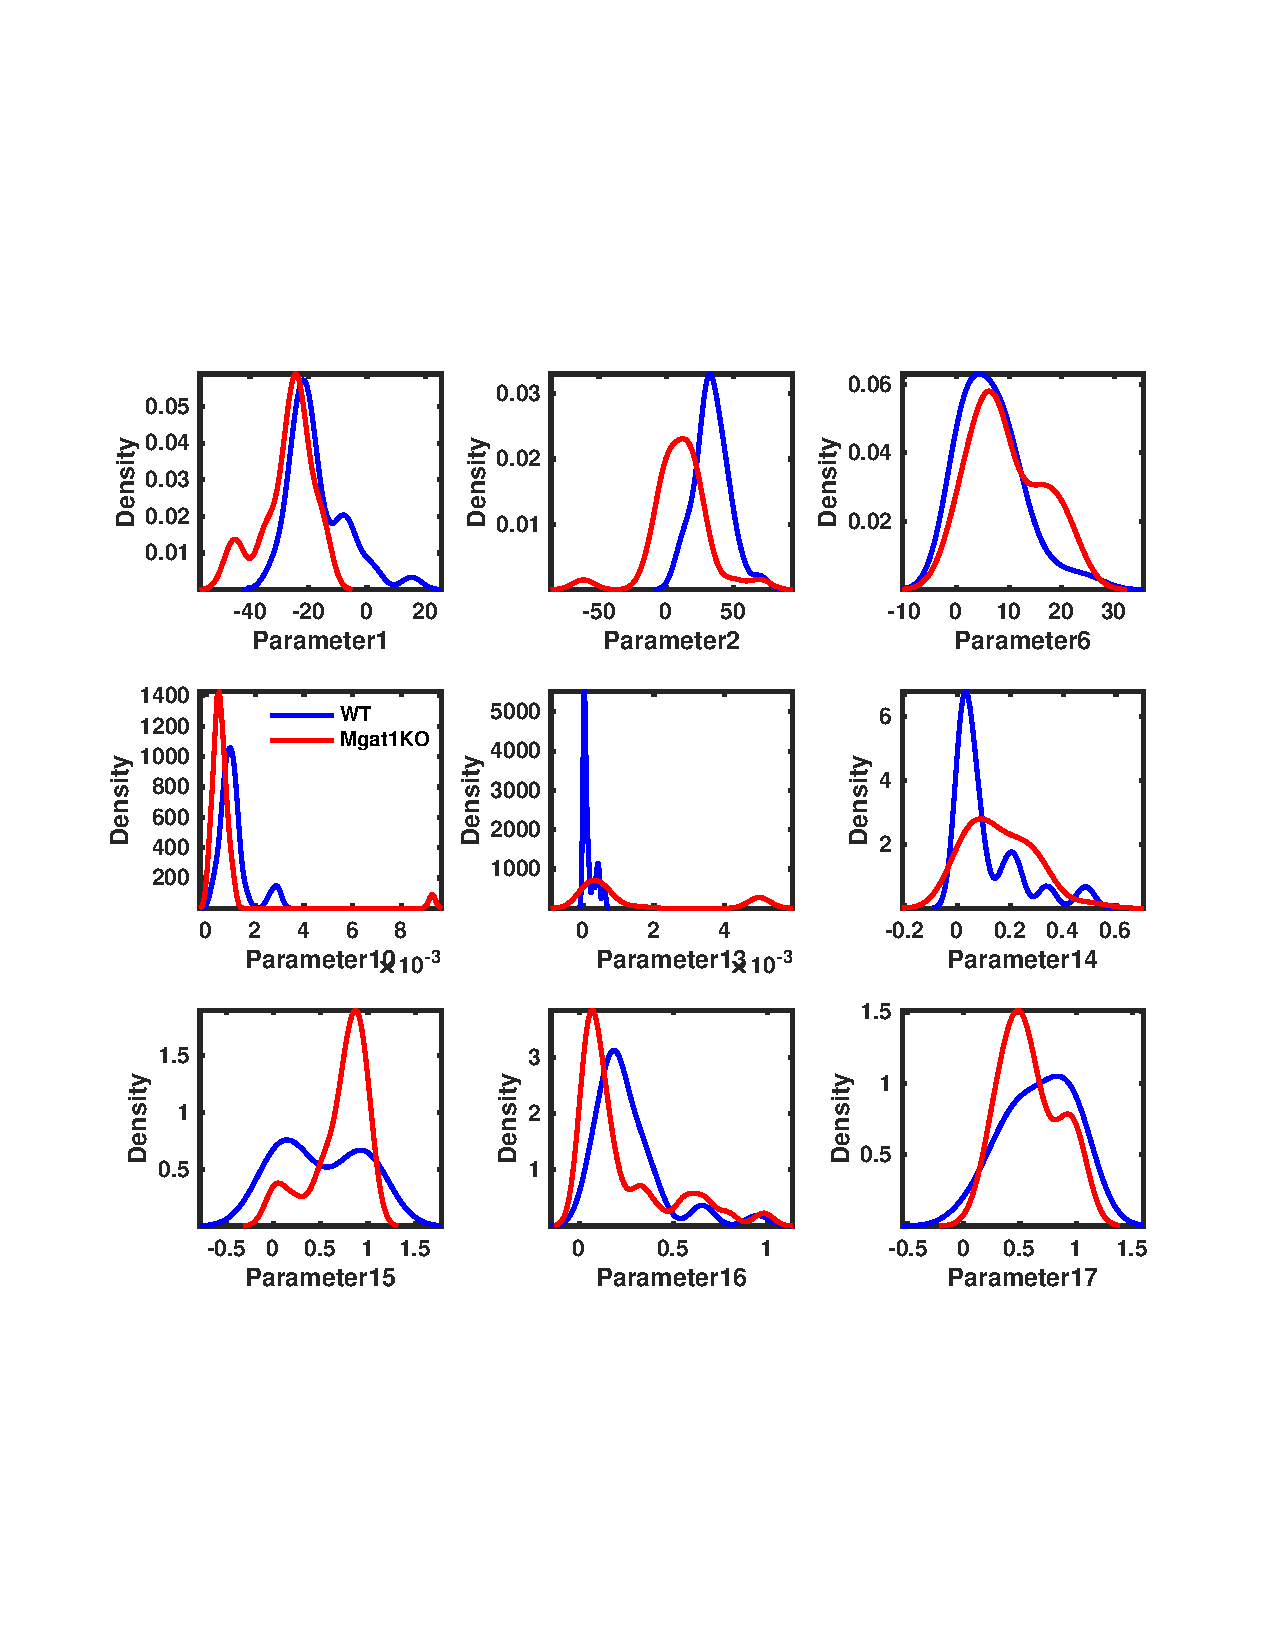
\includegraphics{figs/pkto.pdf}
    \caption{parameter distribution}
    \label{fig:pkto}
\end{figure}

\begin{figure}
    \centering
    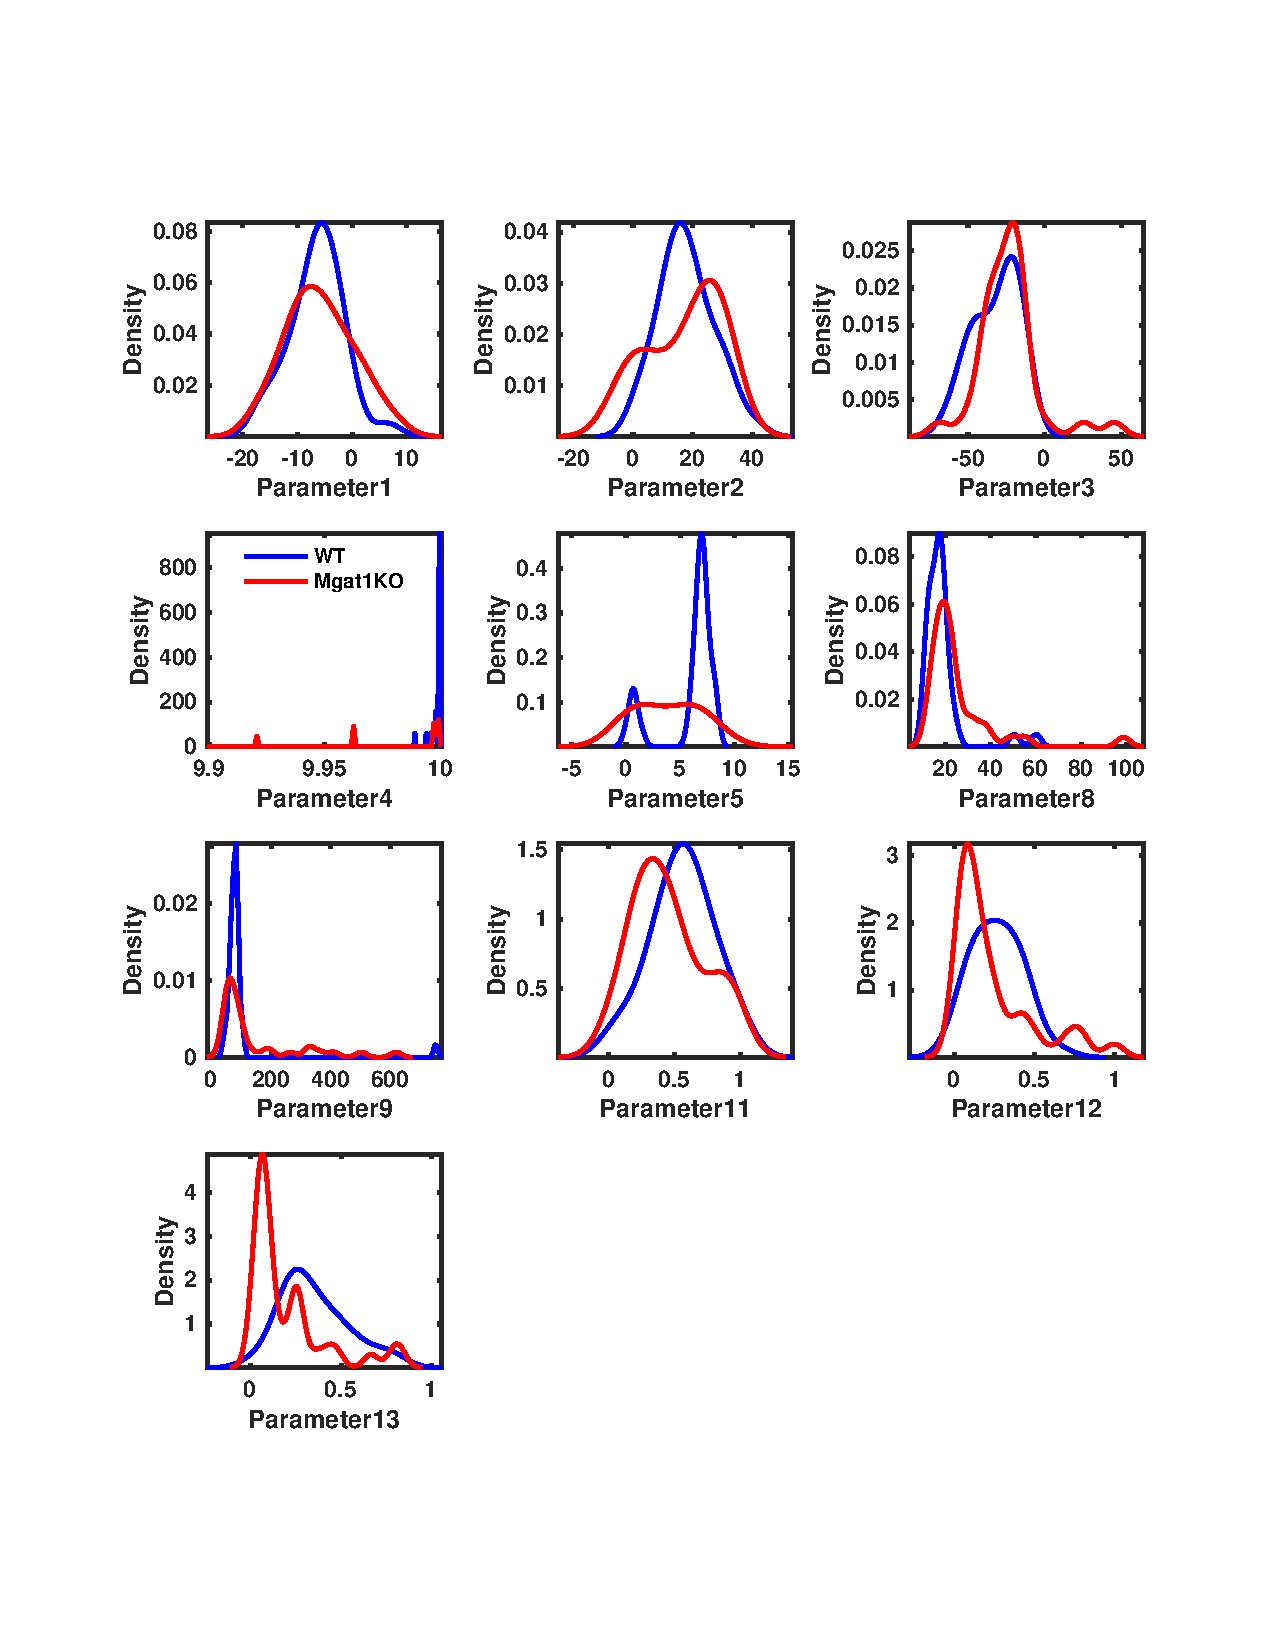
\includegraphics{figs/pkslow1.pdf}
    \caption{parameter distribution}
    \label{fig:pkslow1}
\end{figure}

\begin{figure}
    \centering
    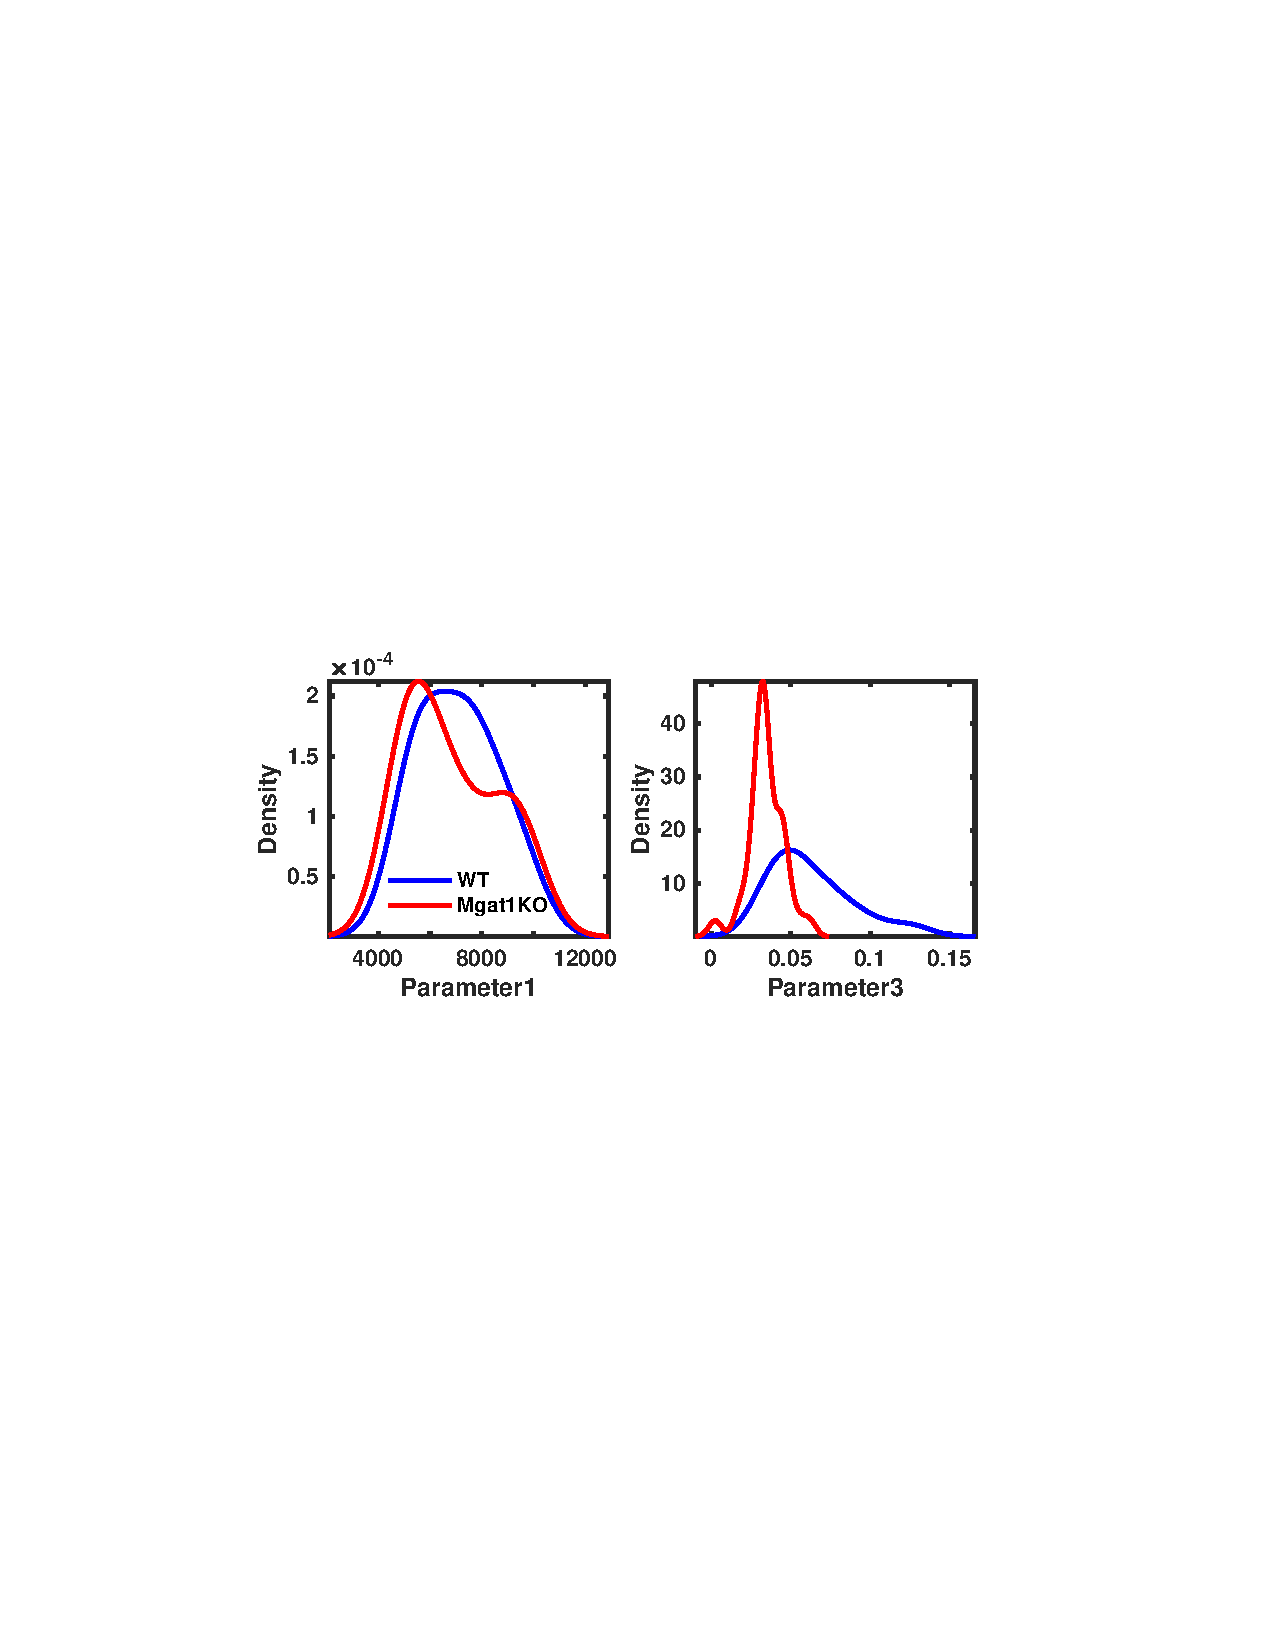
\includegraphics{figs/pkslow2.pdf}
    \caption{parameter distribution}
    \label{fig:pkslow2}
\end{figure}

\begin{figure}
    \centering
    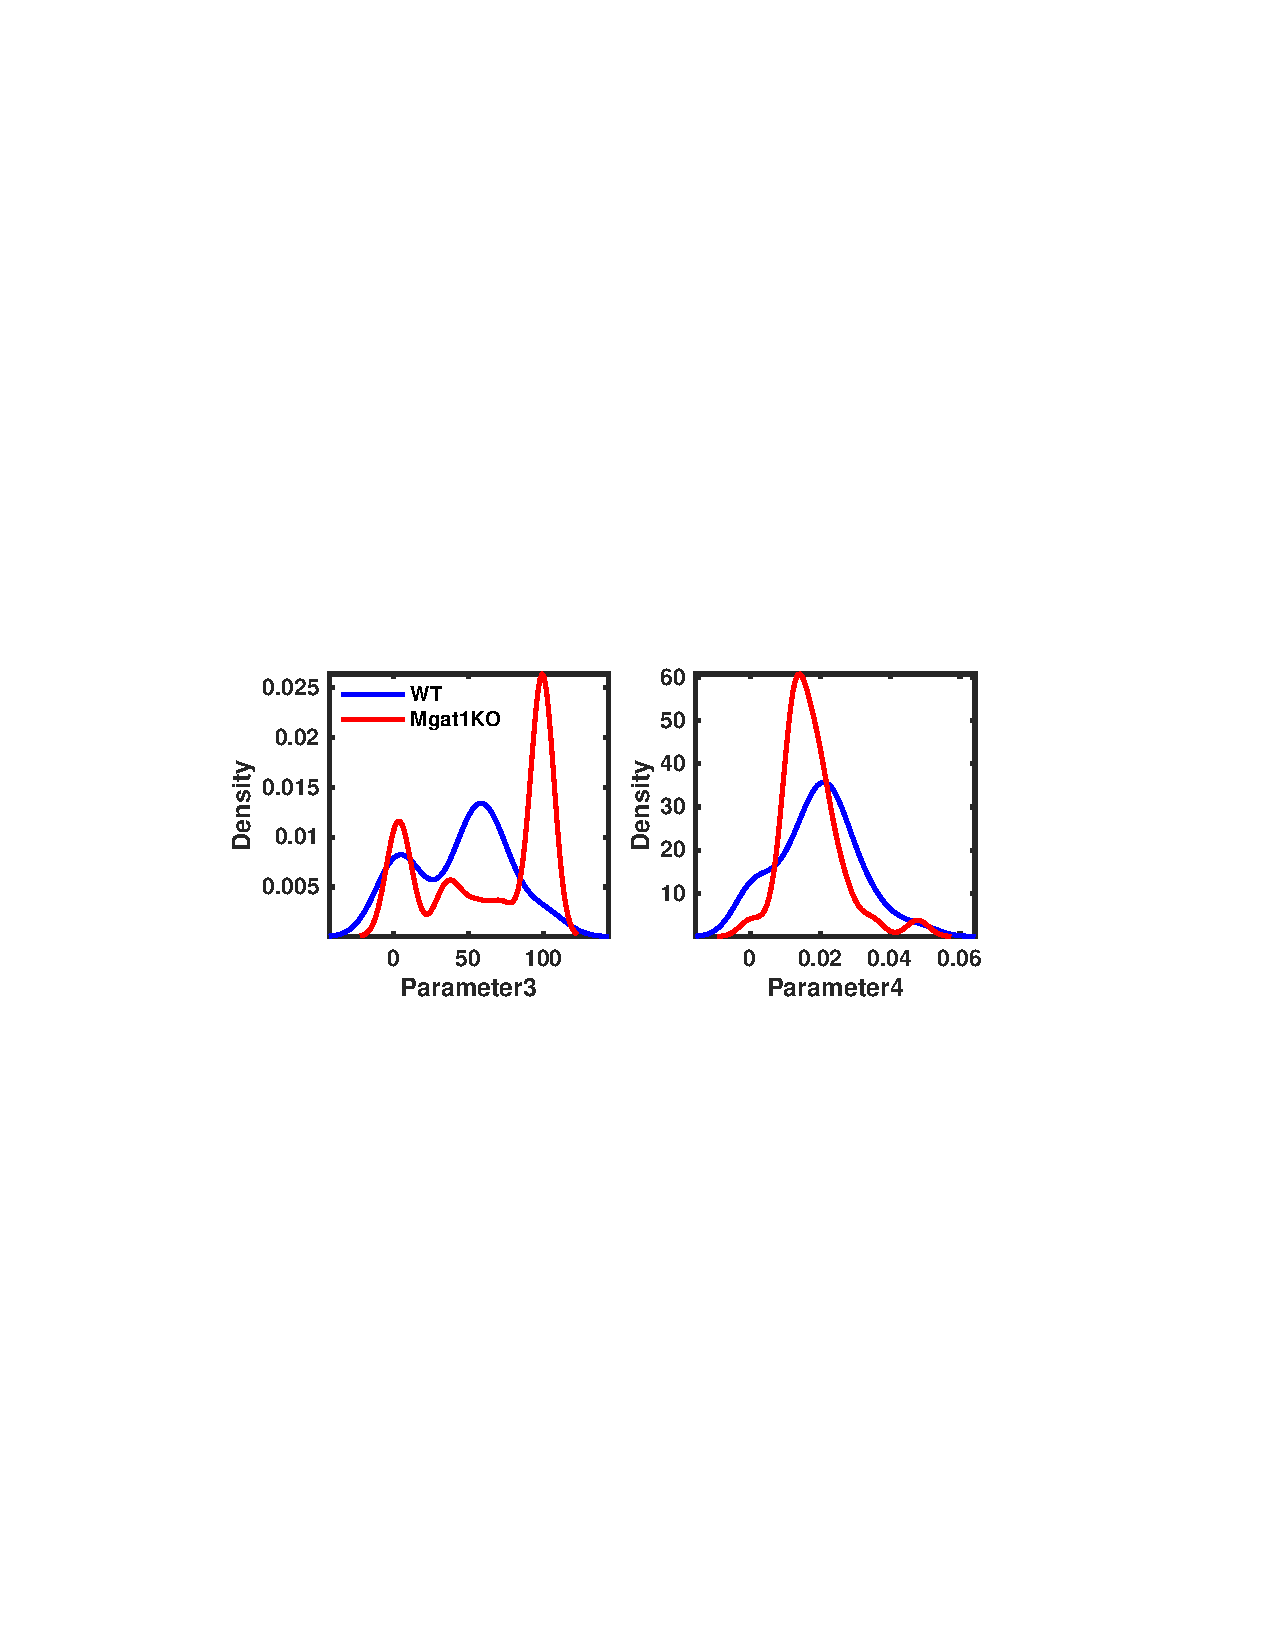
\includegraphics{figs/pkss.pdf}
    \caption{parameter distribution}
    \label{fig:pkss}
\end{figure}

Perhaps numerical analysis of performance, comparison, and demonstration of applicability and impact using real data.

\section{Conclusion}\label{s:conclusion}
A paper ends with a conclusion or summary section.

\if0\blind{
\section*{Acknowledgements}
The authors acknowledge the generous support from the funding agency of XYZ and funding list} \fi

\bibliographystyle{chicago}
\spacingset{1}
\bibliography{IISE-Trans}
	
\end{document}
